\documentclass[12pt]{article}

% set margins and spacing
\addtolength{\textwidth}{1.3in}
\addtolength{\oddsidemargin}{-.65in} %left margin
\addtolength{\evensidemargin}{-.65in}
\setlength{\textheight}{9in}
\setlength{\topmargin}{-.5in}
\setlength{\headheight}{0.0in}
\setlength{\footskip}{.375in}
\renewcommand{\baselinestretch}{1.0}
\linespread{1.0}

% load miscellaneous packages
\usepackage{csquotes}
\usepackage[american]{babel}
\usepackage[usenames,dvipsnames]{color}
\usepackage{graphicx,amsbsy,amssymb, amsmath, amsthm, MnSymbol,bbding,times, verbatim,bm,pifont,pdfsync,setspace,natbib}
\usepackage{multirow, amsmath}
\usepackage[table]{xcolor}

% enable hyperlinks and table of contents
\usepackage[pdftex,
bookmarks=true,
bookmarksnumbered=false,
pdfview=fitH,
bookmarksopen=true,hyperfootnotes=false]{hyperref}
\hypersetup{colorlinks=true, linkcolor=blue, citecolor=blue}

% enable flowchart diagram package
\usepackage{tikz}
\usetikzlibrary{shapes.geometric, arrows}
\usepackage{graphicx}

% define environments
\newtheorem{definition}{Definition}
\newtheorem{fact}{Fact}
\newtheorem{result}{Result}
\newtheorem{proposition}{Proposition}



\begin{document}
\title{Crime and Drug Treatment across Detroit}
\author{Rachel Gaudreau\thanks{Syracuse University, Economics Department. Email: regaudre@syr.edu.} \and Sophia Oritz-Heaney\thanks{Syracuse University, Economics Department. Email: sgortizh@syr.edu} \and Weston Maechling\thanks{Syracuse University, Economics Department. Email: wrmaechl@syr.edu.} \and Leo Gershman\thanks{abc}}
\date{\vskip-.1in \today}
\maketitle

\bigskip
\begin{center} {\bf Abstract} \end{center}

\begin{quote}
    {\small We examine the effects drug and alcohol treatment centers have on their neighbors in Detroit, Michigan. In this study, we find the relationship between the distance from a substance abuse treatment centers and the number of 911 calls in an area. We create a framework that locates all the  substance abuse treatment centers in the greater Detroit area and then creates rings around them at distances ranging from 50 to over 2000 meters to find the number of calls within each ring. Our analysis uses multiple t tests to find the number of calls within a ring and the probability that this is indicative of all crime in the city throughout its history. To complete this, we used a 0.05 confidence interval. This data was found through the City of Detroit's Open Data Portal. Our group looked in the "Police Serviced 911 Calls" section. This portal contains a wealth of information on the type of crime committed along with where and when it was committed. With this information, we were able to make a map using ARCGIS to organize the hundreds of thousands of data points.} 
\end{quote}

\bigskip
\section{Introduction} \label{sec:introduction}
  A common concern among the general American public is that crime rates are increasing. About 6 in 10 Americans share this concern according to Pew Research Center. Additionally, drug usage is another public concern in the American populous, especially in urban centers. This paper seeks to find a correlation between proximity to  substance abuse treatment centers and crime. Our hypothesis theorizes that a closer proximity to substance abuse treatment centers increases access to drug rehabilitation and mental health resources, which, in turn, decreases drug usage. This reduction in drug usage would theoretically lead to a decrease in drug-related crimes and, consequently, fewer calls to 911. So, we explored the question, "How does the distance to the closest drug rehabilitation center relate to the number of calls to 911?" 

Our hypothesis is based on the established impact of drug rehabilitation centers on community well-being . \cite{SAT_centers_and_crime} agrees with this point by showing that there is a decline on all violent crimes within the year of a substance abuse treatment center opening in an area.  Studies such as \cite{drugs_and_crime} and \cite{drugs_crime_space_time} have demonstrated that these centers can lower crime rates and elevate the standard of living in surrounding areas. This means that substance abuse treatment centers can help community well-being by doing more than preventing crime. This is shown in \cite{mental_healthcare_and_crime}, an article showing that drug dependency is a leading cause of criminal behavior. By reducing this dependency, substance abuse treatment centers improve the crime rates in their neighborhoods. The lack of criminal behavior allows people to fully embrace better lives that are closer to their communities further decreasing the amount of 911 calls. 

To explore the relationship between crime and SATC, we conducted a spatial analysis of Wayne County, where Detroit is located. We mapped the locations of drug rehabilitation centers in conjunction with the data points representing 911 calls. Our results showed that areas closer to substance abuse treatment centers had a higher number of 911 calls when compared to areas further away.  Interestingly, further analysis revealed that this trend persisted even when isolating calls related to criminal activities. This shows that while our initial hypothesis on the trend of 911 call density was not support in this data, our insights into the relationship between drug usage and 911 calls could still be possible as stated in \cite{Socioeconomic-Determinants}. 

A potential explanation for these findings could be the reluctance of wealthier communities to give drug rehabilitation centers consent inside their neighborhoods. They could fear that such facilities might attract individuals they perceive as a threat due to their unstable nature as addicts as shown in \cite{mental_health_and_disability}. This "Not in My Backyard" (NIMBY) mentality can lead to fewer treatment centers in areas where they might otherwise reduce crime rates effectively. Instead, treatment centers would be prioritized in areas that already had a high crime rate and a lower standard of living. These places might not be able to perform to their best abilities due to information from \cite{cost_of_drug_treatment}. These places get their funding from the surrounding neighborhoods and a poorer neighborhood means less money and supplies to help the needy. The treatment centers alone wouldn't be able to fully stop this issue immediately and further testing on the impacts of these treatment centers over time could be necessary. 

Answering this question is crucial for developing strategies to mitigate drug-related crimes along with crimes as a whole in American cities. As shown in \cite{SAT_centers_and_crime}, drugs are a major source of civil unrest, social discord, and crime, particularly in urban areas. This is especially true in areas that are historically under supported. By understanding the relationship between treatment center proximity and emergency call frequency, we can work toward solutions that foster safer and healthier communities. Due to this, we will examine whether proximity to drug rehabilitation centers influences crime and 911 call patterns in this paper. Hopefully our work will be able to, offer insights that could guide future policy and urban planning.




\section{Literature Review} \label{sec:literature}
    The geographical relationship between crime and access to mental health care is a widely studied topic but can be convoluted. For example, mental illness is associated with an increased likelihood of substance abuse, which directly and indirectly relates an increase in crime to mental illness. One viable method of treating mental illness is through office-based mental healthcare. Thus, evidence shows that increasing access to office-based mental health care by 10 mental health care provider offices in a county can lead to a 0. 4\% reduction in the county crime rate. \cite{mental_healthcare_and_crime}). An increase in access to mental health care also shows a connection to participation in government disability programs. This is largely because better access to mental health facilities increases the likelihood of proper diagnosis of serious mental illness which leads to access to programs such as Supplemental Security Income (SSI) and Social Security Disability Insurance (SS(D)I). \cite{mental_health_and_disability}. While access to disability insurance does not directly relate to crime this shows that increasing access to mental health care allows for more opportunities for support and better access to the social safety net. Furthermore, this effect is also evident when specifically considering access to substance abuse treatment (SAT) facilities. Evidence shows that increasing access to SAT facilities reduces violent crime due to the effectiveness in reducing crimes motivated by obtaining money to purchase drugs, reducing violence among those in the drug trade, and reducing drug usage which eases aggressive behavior due to drug abuse \cite{SAT_centers_and_crime}. 

However, a significant barrier to treatment could be the price of substance abuse treatment. In a study conducted between 2002 and 2003, the median willingness to pay for drug rehabilitation is shown to be below the average cost of treatment. Moreover, the cost of drug treatment is a significant indicator of self-reported probability of enrollment. \cite{cost_of_drug_treatment}. While it is likely that cost of treatment has changed in the subsequent decades, it is still important to acknowledge barriers to treatment when considering its affects on crime rates in an urban area, such as Detroit. 

Barriers to  treatment also contribute to evidence of a positive feedback loop between drug usage, crime, and standard of living in a given area. The drug trade, specifically the sale and use of drugs in a given area has been closely linked to an increase in the crime rate in the subsequent area. A case study of Miami-Dade county shows that drug activity on a given block can alter or nullify the relationship between household income and crime. Thus, drug usage can be a predictor of crime rates in a geographical area \cite{drugs_crime_space_time}. This effect also has implications on an areas living standards. Since, Higher levels of drug usage leads to higher crime rates in a given geographical area, this corresponds to lower standards of living. This affect is due to the addictive properties of drugs, the numbing of decision making caused by drug usage, and the relationship between areas with lower standards of living and a higher tendency for those who live within such an area to turn to drugs as a means for escape \cite{drugs_and_crime}.

Considering the almost conflicting theories on how drugs, crime, and drug treatment are related and the affects on geographical area, understanding how drug treatment relates directly to crime in the area will give insight into possible policies to reduce crime in an area. Furthermore, given the lack of economic research on this topic we decided to focus on a single case study, in this case, Detroit, and the immediate surrounding communities to analyze the effects drug treatment centers have on crime their surrounding area. Moreover, given our focus on crime it is important to understand the impact the COVID-19 Pandemic had on crime in general. Practices such as Social Distancing and at-home quarantines led people to spend more time in privately occupied spaces. This led to a decrease in the amount of crimes committed in a public setting, such as robbery, homicide, physical violence, etc. However, this also led to an increase in crimes committed in private settings, such as domestic violence \cite{covid_and_crime}. Since, COVID-19 had a varied affect on crime for the purposes of our analysis we decided to limit our study of crime prior to the COVID-19 Pandemic.

\section{Theoretical Analysis}
\label{sec:theory}
This paper assesses the hypothesis that as you get further away from a substance abuse treatment center in Detroit, MI you can expect a higher number of calls to 911. \cite{SAT_centers_and_crime} demonstrate how crime rate is negatively related to the number of substance abuse treatment centers. As more centers open, they can provide treatment to people who were previously unable to receive any due to distance constraints. The paper also showed that this number was found through the likelihood dependency on emergency services decreasing, not just crime. This follows along with what \cite{Socioeconomic-Determinants} found;  lower drug usage in an area causes the people who live there to have more stable and prosperous lives. It shows that as someone frees themselves from drug addiction and increases their socioeconomic standing, they become more productive members of society. This greater access to treatment caused overall crime rates to drop as there was a reduction in crimes motivated by drugs or getting the money to acquire more. We can connect it with the findings of \cite{drugs_and_crime} who found that a decreased drug use in an area has a positive correlation with the change in crime in the same area. This rise in both drug usage and crime causes a negatively related change in the standards of living of that area which they found will again negatively relate to the amount of drug usage restarting the cycle. This framework allowed us to analyze our claim (see Figure 1) that the distance to the closest treatment center will impact the ability to receive treatment, negatively affecting the level of drug use in that area, leading to a positively related effect on drugs-related crimes and also positively effecting the total number of 911. 
\vspace{0.5cm}
\begin{figure}[h!]
\caption{} 
\vspace{0.5cm}
    \scalebox{0.8}{\begin{tikzpicture}[node distance= 4.5cm, auto]
    % Define block styles
    \tikzstyle{process} = [rectangle, minimum width=2.5cm, minimum height=1cm, text centered, draw=black, fill=orange!30]
    \tikzstyle{arrow} = [thick,->,>=stealth]

    % Start of the flowchart (horizontal layout)
    \node (A) [process] {Distance to SAT};
    \node (B) [process, right of=A] {Access to Treatment};
    \node (C) [process, right of=B] {Drug Usage};
    \node (D) [process, right of=C, xshift=-0.4cm] {Drug Related Crime};
    \node (E) [process, right of=D] {Number of 911 Calls};
    
    % Draw dashed arrows (negative correlation)
    \draw [arrow, dashed] (A) -- (B);
    \draw [arrow, dashed] (B) -- (C);
    
    % Draw solid arrows (positive correlation)
    \draw [arrow] (C) -- (D);
    \draw [arrow] (D) -- (E);
\end{tikzpicture}

}
\end{figure}


\section{Data}
\label{sec:data}

\subsection{911 Calls in Detroit Area (Dataset 1)}

This data comes from the City of Detroit Open Data Portal's Police Serviced 911 Calls  \href{https://data.detroitmi.gov/datasets/detroitmi::police-serviced-911-calls/about}{911-Data}. It is generated by the Detroit Police Department's Crime Data Analytics when a call is placed. This data set covers 911 calls that are received by precincts around the Detroit metropolitan area from the year 2016-2022. We isolated the observations to one year, 2017, from the original dataset 911-Data so we could perform cross-sectional analysis. This dataset is referred to as 2017-911-Calls. We chose observations from 2017 since the year a) overlaps with dataset 2 and b) is before COVID-19, where crime rates statistics shifted in general \cite{covid_and_crime}. This is to eliminate COVID-19 effects from affecting our data analysis. We used the longitude and latitude variables from 2017-911-Calls for cross-sectional-analysis with treatment-center dataset.

\subsection{Substance Abuse Treatment Centers (SATC) in Detroit Area (Dataset 2)}

This data is from the Substance Abuse and Mental Health Services Administration (SAMHSA). Data is generated through the National Survey of Substance Abuse Treatment Services \href{https://www.samhsa.gov/data/data-we-collect/n-ssats-national-survey-substance-abuse-treatment-services}{N-SSATS} an annual survey of all known public and private substance abuse treatment services in the United States. SAMHSA conducts this survey annually. This data covers the names and addresses of substance abuse treatment services in operation in the Detroit Metropolitan area between the years 2015 to 2021. 


We used the ArcGISPro application to layer both 2017 datasets and geocode their locations. Using the coordinates (longitude and latitude variables) of each point, we created two new variables. Every 911 call is assigned one SATC, the one geographically closest to it. This means no observation is counted twice. 

We used Stata 18.0 to identify distance buckets, referred to as distance groups, and perform our analysis. We standardized the data to account for how different in total area of a distance group might alter results. We did this by dividing the area by the total count of 911 calls in each distance group. 

%Describe your data. Where you got it from, how it was generated, what variables you'll use, what data cleaning steps you had to take, where your processed data, code and documentation is stored.
%In a published paper, a lot of this detail will be in a data appendix. For the purposes of this report, include it all here (this may be the longest section of your report).

\subsection{Survey data}

\section{Results}
\label{sec:result}

\begin{figure}[ht]
    \centering
    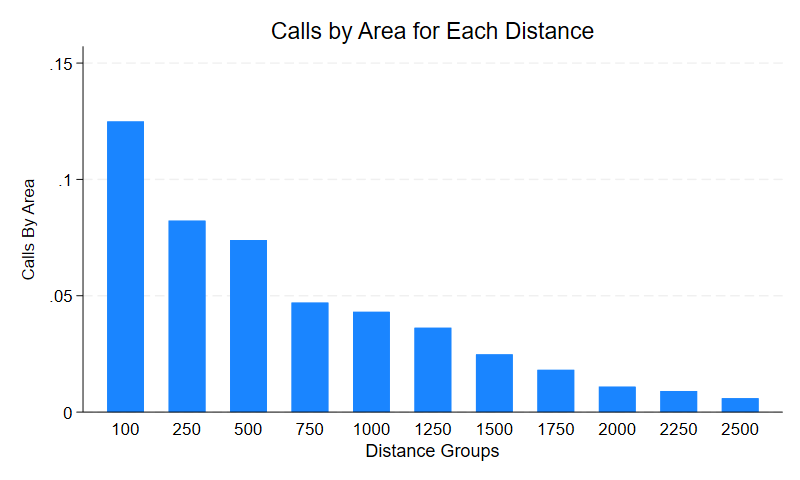
\includegraphics[width=1\linewidth]{Reproducibility Package//Visual Graphics/Avg_Calls_per_Distance_Group.png}
    \caption{Enter Caption}
    \label{fig: Average Number of Calls per Distance Group}
\end{figure}
For the research question "How does the distance to the closest drug rehabilitation center relate to the amount of calls to 911?" our group hypothesized that as the distance from a drug treatment facility increases, the number of 911 calls also increases. This means that the further someone is from a treatment center, the less access they have to treat drug addiction, so the more likely they would exhibit drug-induced behavior that results in someone calling 911. Our null hypothesis is that there is no relation between distance to a drug treatment center and the likelihood of calling 911. 
\begin{figure}[h]
    \centering
    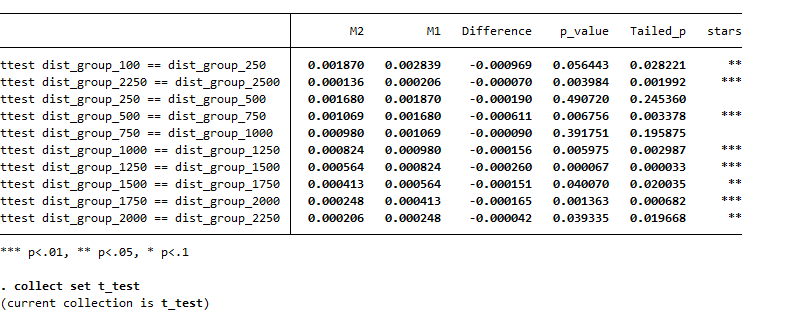
\includegraphics[width=1\linewidth]{Reproducibility Package//Visual Graphics/t_test_ss.png}
    \caption{Two Sample T-Tests}
    \label{fig:enter-label}
\end{figure}
Our data analysis supports the conclusion that the amount of 911 calls increases the closer they are to an SATC. Figures 2 and 4 show a distribution of mean 911 calls per distance group. In Figure 2, the unit of analysis was the mean 911 calls, but with almost 500,000 observations since the data was per 911 call. We conducted a two-sample t-test, seen in Figure 3, between sequential distance groups. 

The results identify that there is statistical significance between most distance group's call averages. However, most of the confidence intervals were extremely high due to the total amount of observations. 5 of the t tests had a p value less than 1\% and 2 of the t test had a p value less than 5\%.  

We revised our graph to account for this potential skewed-ness in the confidence intervals to group the 911 calls count in each distance group by the SATC-assigned variable (, creating 44 total observations (one observation for each SATC). The results are in Figure 4. The confidence intervals show that overall, there is statistical significance in the mean calls of each distance group. The only exceptions are: differences by using the SATC as a group variable, and the We due to high In. The high confidence interval of these sections indicates that there is a strong correlation between distance to a treatment center and the likelihood of a 911 call.

 

\begin{figure}[ht]
    \centering
    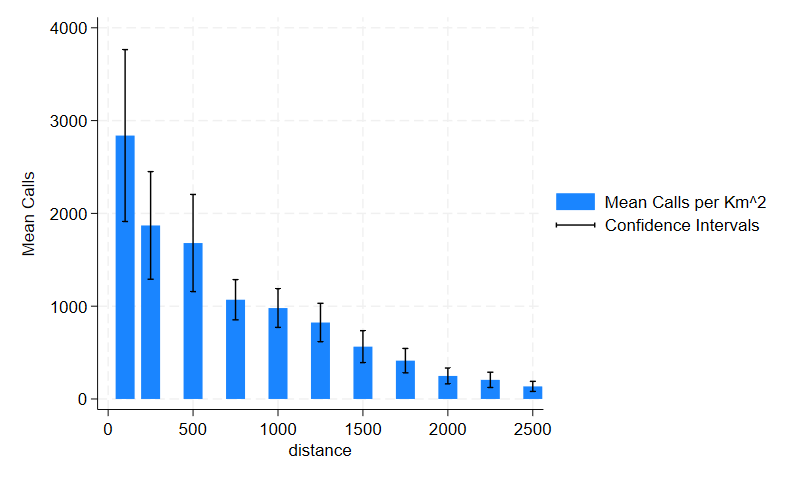
\includegraphics[width=1\linewidth]{Reproducibility Package//Visual Graphics/CI_Graph.png}
    \caption{Mean Calls}
    \label{fig:enter-label}
\end{figure}

\begin{table}[h]
\centering
\caption{Ratio Analysis}
\begin{tabular}{l||c|c|cc|c|c}
\hline\hline
            &ratio\_results&            &            &            &            &            \\
            &       Ratio&   Std. Err.&  [95 Conf.&   Interval]&     T score&     P value\\
\hline
100/250     &    1.518016&     .305492&     .901933&      2.1341&    4.969087&    .0000112\\
250/500     &    1.112848&    .1703623&    .7692794&    1.456416&    6.532241&    6.14e-08\\
500/750     &    1.571244&    .1966827&    1.174596&    1.967893&    7.988725&    4.92e-10\\
750/1000    &    1.091451&    .1104992&    .8686081&    1.314294&    9.877456&    1.25e-12\\
1000/1250   &    1.189354&    .0748615&    1.038382&    1.340327&     15.8874&    1.32e-19\\
1250/1500   &    1.461179&    .1268808&    1.205299&    1.717058&    11.51615&    1.00e-14\\
1500/1750   &    1.365242&    .1935897&    .9748308&    1.755652&    7.052244&    1.08e-08\\
1750/2000   &     1.66361&    .2204068&    1.219117&    2.108103&    7.547907&    2.09e-09\\
2000/2250   &    1.204906&     .110774&    .9815093&    1.428303&    10.87716&    6.33e-14\\
2250/2500   &    1.519659&    .1688579&    1.179124&    1.860193&     8.99963&    1.91e-11\\
\hline\hline
\end{tabular}
\flushleft
\begin{footnotesize}
\begin{singlespace}
\textbf{Note 1}: A larger T score indicates the estimated coefficient is more significantly different from the hypothesized value.
\textbf{Note 2}: A smaller P value p<0.05 means the result is statistically significant. This means the estimated coefficient is likely not zero.
\end{singlespace}
\end{footnotesize}
\end{table}

%\subsubsection{Summary Statistics}
%State your working hypothesis and null hypothesis - Explain why the statistics you’re presenting are appropriate -Present statistics and explain what they mean (e.g., do your results support the working hypothesis? 

%Explain what analyses you did, provide evidence (like in the descriptive stats exercise, but refined and clear) and then explain what your results mean.


\section{Discussion}
\label{sec:discussion}

One explanation for this relationship could be due to the positive feedback loop between drugs, crime, and lower standards of living in those places. Drug treatment centers may be purposely selected in drug usage hot spots, which tend to have other associated demographics such as high population density and lower standard of living. These communities tend to have higher crime rates in general, which could explain part of this trend. Alternately, they may be placed there since higher standards of living communities, which tend to have lower crime rates in general, will rally against SATC being placed in their neighborhoods, due to fear of the type of people it will bring to the neighborhood. 
    
Another explanation for the lower frequency of 911 calls in further distance rings could be due to our data not counting 911 calls twice. When we geo-coded the 911 calls, we assigned each observation to only one SATC, the one geographically closest to it. This was to limit the amount of overlap that some SATC might have at the smaller distance rings, as it could exaggerate our data frequencies. However, in farther distance rings, a call might be similar in distance to two SATCs, but will only be assigned to be correlated to one, when the reality it could be correlated to either. This thins the observations and data associated in farther-out distance rings. 

One significant limitation was the inability to fine-tune 911 call data to determine whether calls were directly related to drug activity. Without additional data, such as toxicology reports or detailed incident descriptions, it remains challenging to assess the role of drugs in criminal behavior or whether the crimes involved were violent in nature. A better understanding of what calls were drug-related or induced could provide more accurate results on the relationship between drug abuse and crime, and the role of SATC in amplifying or mitigating this. 
    
Another limitation is the population density of this urban sample. The observed pattern of 911 calls could have been influenced by higher population density in more urban parts of Detroit, which naturally results in an increase of emergency calls. Future research should explore similar analyses in areas with varying population densities to better control for this variable and isolate the effects of proximity to drug treatment centers. 

Another limitation was the inability to create a regression line (or line of best fit) for this relationship. Since we collapsed the data multiple times, we lost variability to perform a regression line. First, we collapsed the data by count to get the total counts for each distance group. Then we collapsed the data by grouping by SATC designation, to get the total observations per distance group per SATC. Finally, we collapsed that data set by mean, creating mean counts of 911 calls per distance group adjusted for SATC correlation. This left one observation row that created Figure 4. We lost analysis flexibility due to this data manipulation approach. In the future, a different data manipulation approach might leave more room for further data analysis. 

\section{Conclusion}
\label{sec:conclusion}

    We hypothesized that as the distance from a substance abuse treatment center (SATC) increases, the frequency of 911 calls also increases. The closer a SATC is, the more accessible treatment centers are, which should reduce crime rates in the area, measured by 911 calls. We conducted a cross-sectional analysis to examine the overlap of 911 calls' geographical locations to their distances to their closest SATC. Our results show that contrary to our hypothesis, as distance from a SATC increases, the amount of 911 calls decreases. This distance decay relationship indicates that there is a relationship between SATC placements and 911 calls, but just in the opposite direction of the original hypothesis. 
   % A


 
%Re-state (in different words) what you did and what you learned. If your discussion (Section 6) would be short, you can just have a Conclusion section that includes your discussion (that is, leave out a separate Discussion section).

\newpage
\singlespacing
\setlength\bibsep{0pt}

\bibliographystyle{chicago}
\bibliography{reference.bib}
https://www.pewresearch.org/short-reads/2024/04/24/what-the-data-says-about-crime-in-the-us/

\newpage
\section*{Data Appendix} \label{sec:appendixa}
\addcontentsline{toc}{section}{Appendix A}

You should at least direct your reader to your replication package. You might put key elements of your replication package in this section as well.

\end{document}